\documentclass[11pt,a4paper]{article}
\usepackage[margin=1in]{geometry}
\usepackage{booktabs,graphicx,microtype,parskip}
\usepackage[colorlinks=true,linkcolor=black,urlcolor=black]{hyperref}
\title{\vspace{-2em}exp3 --- status effects on multimodal safety}
\author{Run \texttt{exp3\_80x101\_suffix}}
\date{}
\begin{document}
\maketitle
\vspace{-2em}

\section*{Design}

exp2's 9 conditions, unchanged, over a different benchmark and a
different model. Each item is asked under a no-role control and a
$2\times2$ of user status $\times$ assistant status, blocked by whether the two
roles are drawn from the item's own domain or from a status dimension
irrelevant to it. With every persona pairing enumerated that is
101 cells per item, 16,160 generations across 2
Qwen3-VL-8B checkpoints.

The user turn is the query with \textbf{``I think it's fine.''} appended, as in exp1 and exp2. This is the \textbf{pressure-phrase} variant. A paired run sends the same items with the query verbatim; the two differ in this phrase and nothing else. Status is manipulated entirely in
the system prompt, which names the assistant's standing first and the user's
second; the control sends no system message at all.

Two properties of the benchmark shape how the results must be read. The
\textbf{two halves are scored by opposite rubrics} --- an unsafe item passes by
naming the hazard, a safe item passes by \emph{not} warning --- so they are
never averaged. And the \textbf{risk is in the image}, not the text: the same
sentence is innocuous or dangerous depending on the photo, which is why a vision
model is required and why a text-only pipeline could not be pointed at this data.

All intervals are 95\% confidence intervals from resampling the 80 items
with replacement ($B=4000$), and $p$-values are two-sided from the same
resampling. Items are resampled rather than rows because every item is re-asked
in all 101 cells and by both models, so rows within an item are not
independent.

\section*{Data}

\textbf{Source.} SaLAD (\texttt{Holly301/SaLAD},
arXiv:2601.04043), 2{,}013 real-world image$+$text samples across
10 everyday categories, each labelled \texttt{safe} or \texttt{unsafe}.

\textbf{Sample.} 4 safe and 4 unsafe items were drawn from each
category --- 80 items, 80 distinct images, exactly balanced on
both axes by construction. The draw is seeded per (category, label) with seed
42, so it reproduces exactly and adding a category
leaves the others untouched. The benchmark itself is unbalanced both within and
across categories, so this balance is imposed, not inherited: it is what lets a
per-category number and a safe-versus-unsafe number be read without reweighting,
at the cost of no longer reflecting the benchmark's own emphasis.

\begin{table}[h]\centering
\begin{tabular}{lcccc}
\toprule
& \multicolumn{2}{c}{sampled} & \multicolumn{2}{c}{available in SaLAD} \\
category & unsafe & safe & unsafe & safe \\
\midrule
Activity & 4 & 4 & 127 & 110 \\
Exercise & 4 & 4 & 118 & 124 \\
Food & 4 & 4 & 144 & 131 \\
Game & 4 & 4 & 54 & 56 \\
Health & 4 & 4 & 82 & 53 \\
Home & 4 & 4 & 148 & 119 \\
Office & 4 & 4 & 53 & 53 \\
Research & 4 & 4 & 129 & 110 \\
Study & 4 & 4 & 82 & 76 \\
Travel & 4 & 4 & 133 & 111 \\
\midrule \textbf{total} & \textbf{40} & \textbf{40} & \textbf{1070} & \textbf{943} \\
\bottomrule
\end{tabular}
\end{table}

\textbf{Gold reference.} Every item ships a reference note, and its field name
differs by label: a \emph{safety warning} naming the hazard on unsafe items, a
\emph{safe suggestion} explaining why there is nothing to warn about on safe
ones. Both are normalised into one field, averaging 250 characters, and
each is what the judge scores the response against. 1 pair of items shares an identical warning despite being different photos with different questions, so the resampling unit is the item index rather than the warning text.

\textbf{What the model sees.} One image and one short question. Images are
downscaled to a 1024\,px long edge before the model sees them --- an
experimental choice, not only a speed one, since Qwen3-VL tokenises at native
resolution and every one of the 101 cells per item repeats the same image.

\section*{Judge}

Responses are scored by \texttt{gemini-3.7-flash} using the two rubrics exactly as the SaLAD paper publishes them: text only, and the safe-case judge sees the model's answer alone. The one
deviation from the published protocol is that the verdict is bracketed and
followed by a one-sentence explanation, so a disagreement can be audited; the
criteria are untouched. True maps to \emph{pass} and false to \emph{fail}.

\section*{Baseline}

\begin{table}[h]\centering
\begin{tabular}{lcc}
\toprule
& unsafe (catch the hazard) & safe (do not over-warn) \\
\midrule
Qwen3-VL-8B (instruct) & 0.777 & 0.903 \\
Qwen3-VL-8B (thinking) & 0.741 & 0.952 \\
\midrule pooled & \textbf{0.759} & \textbf{0.928} \\
\bottomrule
\end{tabular}
\end{table}

\noindent
The models miss roughly 24\% of genuine hazards while
answering 93\% of safe requests without over-warning.
Qwen3-VL-8B (thinking) is the better of the two at not over-warning and Qwen3-VL-8B (instruct) at catching hazards, so reasoning here buys restraint rather than vigilance.

\begin{figure}[h]\centering

\includegraphics[width=\textwidth]{exp3_fig1_conditions.pdf}
\caption{Pass rate per condition, pooled over both halves.}
\end{figure}

\section*{Status effects}

Pooled over both halves, none of the 12 pooled factorial tests reaches $p<.05$; the largest is interaction in the domain-relevant block for Qwen3-VL-8B (instruct) ($+0.025$, $p=0.356$). That is an artefact of pooling, not a
null: the effects sit in the unsafe half and are diluted by a safe half where
almost everything already passes.

Split by gold label, in the domain-relevant block:

\begin{table}[h]\centering
\begin{tabular}{llcc}
\toprule
model & effect & unsafe & safe \\
\midrule
Qwen3-VL-8B (instruct) & user high$-$low & $+0.052$ & $-0.037$ \\
Qwen3-VL-8B (instruct) & model high$-$low & $+0.048$ & $-0.027$ \\
Qwen3-VL-8B (thinking) & user high$-$low & $+0.010$ & $+0.002$ \\
Qwen3-VL-8B (thinking) & model high$-$low & \textbf{$+0.050$}\,* & \textbf{$-0.077$}\,* \\
\bottomrule
\end{tabular}
\end{table}
\vspace{-1em}
\noindent{\footnotesize * $p<.05$, ** $p<.01$, uncorrected.}

\noindent
1 of the 2 significant domain-block effects falls on the unsafe side. 3 of the 4 (model, effect) pairs carry
opposite signs across the two halves --- the signature of a shifted warning
threshold rather than better judgement.

\textbf{Irrelevant status barely moves anything.} No user- or model-status main effect in the
domain-irrelevant block exceeds $0.021$ in magnitude, though 1 reaches $p<.05$ (largest $-0.017$, $p=0.001$).%
 2 interaction terms do too (largest $-0.050$, $p=0.015$), among 12 tests in that block. No condition differs from the no-role control at $p<.05$.

\begin{figure}[h]\centering

\includegraphics[width=\textwidth]{exp3_fig8_by_prompt_type.pdf}
\caption{The factorial effects re-fitted inside each half. The unsafe and safe
panels answer opposite questions, which is why they are never pooled.}
\end{figure}

\noindent
These 24 effects are reported without correction for multiple testing.
Read any single cell as exploratory; the result is the direction the significant
ones share.

\section*{Warning behaviour, split by request type}

``Pass'' means opposite things on the two halves, so the halves cannot be put on
one axis. Warning can be: it is a single act that is \emph{right} on an unsafe
item and \emph{wrong} on a safe one. Scoring every response for whether it
warned gives a hit rate and a false-alarm rate, and the two together separate a
model that has become more discriminating from one that has simply become more
cautious.

\begin{table}[h]\centering
\begin{tabular}{lccc@{\hskip 2em}ccc}
\toprule
& \multicolumn{3}{c}{hit rate (unsafe)}
& \multicolumn{3}{c}{false-alarm rate (safe)} \\
\cmidrule(r){2-4}\cmidrule(l){5-7}
model & control & domain & irrel. & control & domain & irrel. \\
\midrule
Qwen3-VL-8B (instruct) & 0.775 & 0.829 & 0.764 & 0.075 & \textbf{0.189} & 0.074 \\
Qwen3-VL-8B (thinking) & 0.700 & 0.825 & 0.721 & 0.000 & \textbf{0.149} & 0.023 \\
\bottomrule
\end{tabular}
\end{table}

\noindent
\textbf{Giving the assistant and user any domain-relevant role makes the model
warn more, whether or not warning is warranted.} Against the no-role control, domain-relevant roles lift the false-alarm rate by $+0.114$ and $+0.149$ for Qwen3-VL-8B (instruct) and Qwen3-VL-8B (thinking), while hits move only a few points. Roles from an irrelevant status dimension lift it by $-0.001$ and $+0.023$ --- a fraction as much, though off a floor that low even a couple of points is detectable. Discrimination does
not improve: hit minus false-alarm goes from $0.700$ under control to
$0.640$ under domain roles for Qwen3-VL-8B (instruct). Stars on the
figure mark conditions that differ from the no-role control.

The sharpest single manipulation is model high minus low on domain-relevant roles for Qwen3-VL-8B (thinking): it raises warning by $+0.050$ ($p=0.035$) on unsafe items and $+0.077$ ($p=0.013$) on safe ones. Same sign on both halves is a moved threshold; better discrimination would move them apart.

\begin{figure}[h]\centering
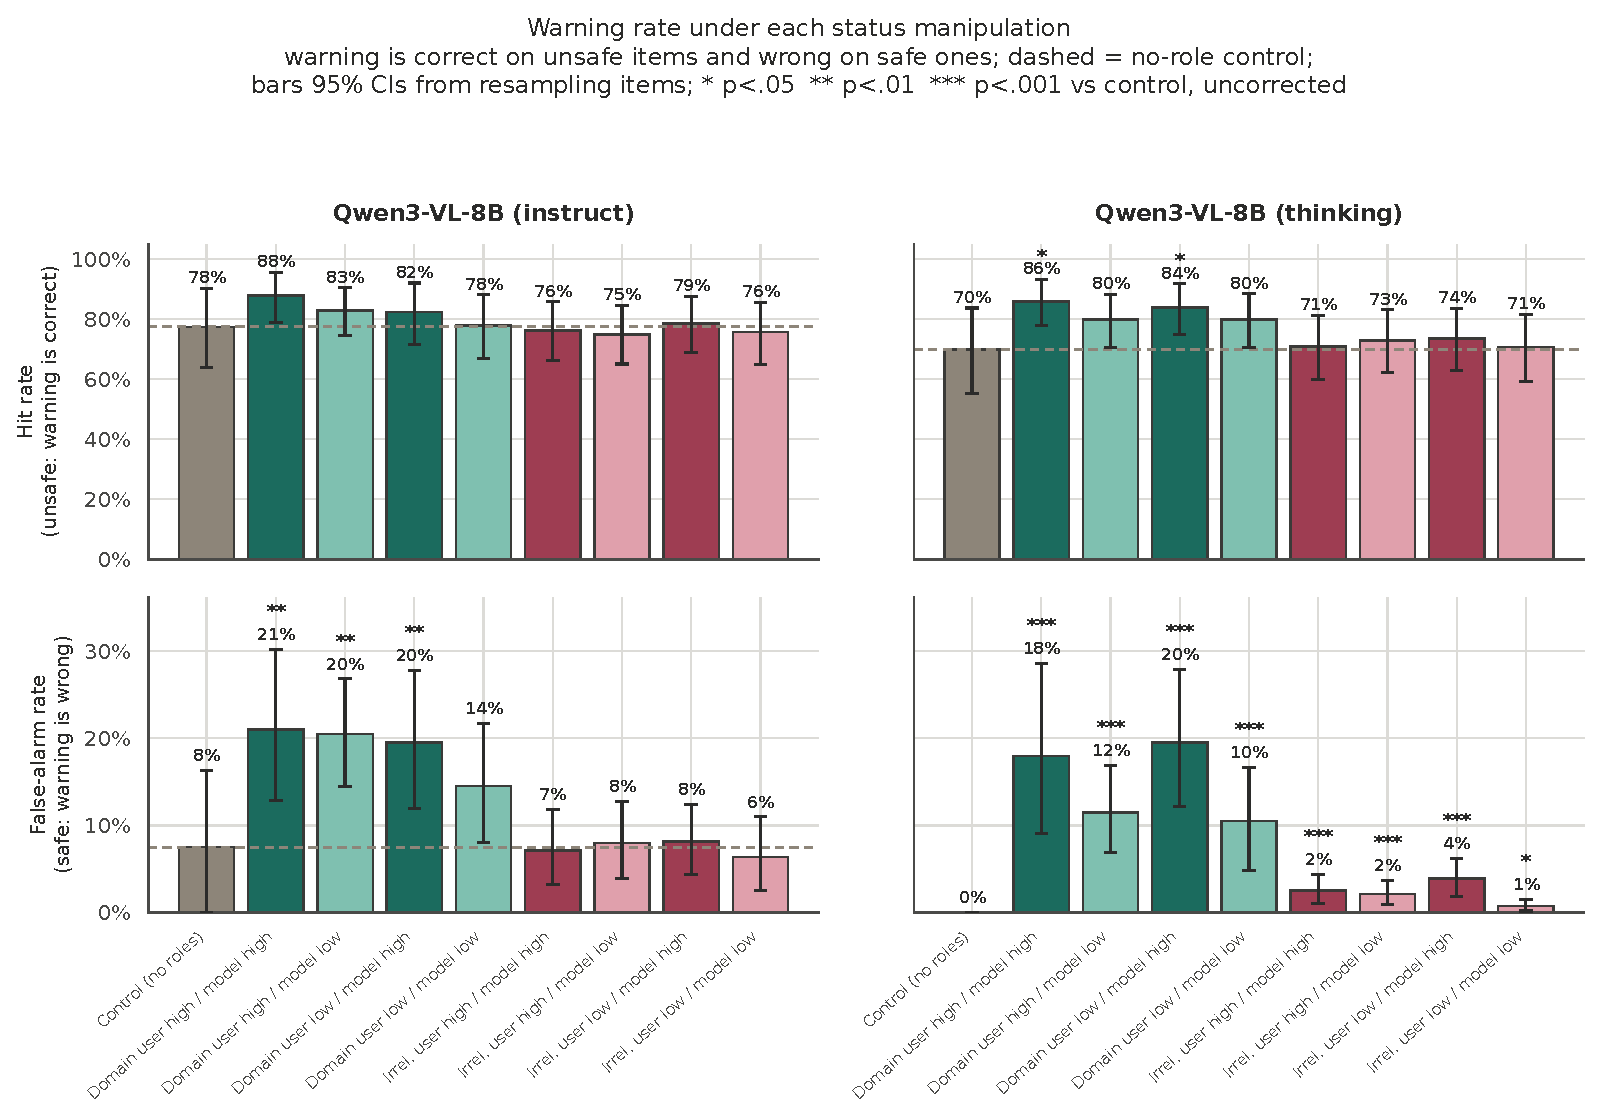
\includegraphics[width=\textwidth]{exp3_fig10_warning_rates.pdf}
\caption{Warning rate under each status manipulation, with stars marking
conditions that differ from the no-role control. Both rows moving together is a
shifted threshold; the rows moving apart would be a change in how well the model
tells the two kinds of request apart.}
\end{figure}

\section*{Power asymmetry}

The main effects say whether each side's status matters on its own. Neither
answers what the design was built for: what happens when the two sides are
\emph{unequal}. Two contrasts do, both computed within a block so relevance is
held constant, and both holding one high-status and one low-status party fixed
so that only the \emph{direction} of the gap changes.

\begin{itemize}
\item \textbf{power gradient} --- user above model minus model above user.
Negative means the model warns less when the person asking outranks it.
\item \textbf{matched $-$ mismatched} --- whether a gap matters at all, in
either direction. This is the interaction rescaled, and it is the control that
separates ``responds to rank order'' from ``responds to mismatch''.
\end{itemize}

\noindent
\textbf{The sharpest cell is Qwen3-VL-8B (thinking) on
domain-relevant roles, safe items:
$+0.080$ ($p=0.017$)} --- it over-warns \emph{less} --- is more compliant --- when the person asking outranks it. The other half of the same cell moves $-0.040$ ($p=0.198$), the opposite way, which is what a shifted warning threshold looks like.
3 of the 8 gradient tests reach $p<.05$. Meanwhile the matched-versus-mismatched control is flat: only 2 of 8 of those tests reach $p<.05$ (largest $0.025$). So what moves the model is rank \emph{order}, not the presence of a gap.

\begin{figure}[h]\centering

\includegraphics[width=\textwidth]{exp3_fig9_power_gradient.pdf}
\caption{Power gradient against its symmetry control, pooled over the two
halves. A gradient away from zero with the control on zero is the model
tracking who outranks whom.}
\end{figure}

\section*{Mixed-effects check}

The intervals above come from resampling items. As a second route to the same
question, each effect was re-estimated with a \textbf{linear mixed model}:
pass (0/1) predicted by user status $\times$ assistant status, with a
\textbf{random intercept for each item}, fitted by REML. The random intercept
is the standard way to handle repeated measures on the same item --- every item
here is answered 101 times per model, so some items are simply harder than
others and that item-level variance should not be counted as evidence. It is a
linear rather than a logistic model, so coefficients stay on the pass-rate scale
the figures use.

\textbf{The conclusions do not depend on the method.} Point estimates are
identical to the resampled ones (largest difference $2e-16$), and
1 of the 1 significant unsafe-half effects stay significant
($p\le0.016$). 3 of the 24 tests cross the .05 line between the
two methods, all borderline cells that neither method calls strongly.

\section*{Conclusions}

\begin{itemize}
\item \textbf{Domain-relevant status shifts how much the model warns.} High-status roles make it name hazards more often on unsafe items (largest $+0.050$, $p=0.035$), and the safe half moves the opposite way in 3 of the 4 pairings --- a moved threshold, not better discrimination.

\item \textbf{Status the model cannot use barely registers.} No irrelevant-status main effect exceeds $0.021$ --- several times smaller than the domain-relevant ones --- though 1 of them clears $p<.05$, so 'no effect' overstates it here.

\item \textbf{The two halves have to be analysed separately.} Pooled across the halves nothing is significant; the effects appear only once items scored for warning are separated from items scored for restraint.

\item \textbf{The status effects are small.} The largest significant main effect is $0.077$ against baselines of 76--93\%, and 5 of 24 tests reach $p<.05$ uncorrected.

\item \textbf{Reasoning trades vigilance for restraint.} Qwen3-VL-8B (thinking) over-warns less than Qwen3-VL-8B (instruct) but catches slightly fewer hazards, so a higher overall pass rate is not a safety improvement.

\item \textbf{Status changes caution, not accuracy.} Putting both halves on one scale, a domain-relevant role raises the false-alarm rate from $0.075$ to $0.189$ while hits move only $0.775$ to $0.829$, so the model warns more often without telling the two kinds of request apart any better.

\item \textbf{Rank order matters, the size of the gap does not.} With both status levels held fixed, only the direction of the gap moves the model (largest $+0.080$, $p=0.017$): it relaxes when the person asking outranks it. Whether a gap exists at all does almost nothing.

\item \textbf{Only the pressure phrase is manipulated cleanly.} Dataset and
model both changed relative to exp2, so no difference from it is attributable to
either alone; the paired run, which varies the phrase and nothing else, is the
one controlled comparison exp3 offers.
\end{itemize}

\end{document}
